\documentclass[conference]{IEEEtran}
\IEEEoverridecommandlockouts

\usepackage{cite}
\usepackage{amsmath,amssymb,amsfonts}
\usepackage{graphicx}
\usepackage{textcomp}
\usepackage{xcolor}
\usepackage{booktabs}
\usepackage{array}
\usepackage{tikz}
\usetikzlibrary{arrows.meta,positioning}
\usepackage[hidelinks]{hyperref}

% Placeholder: a value that must be supplied by the authors before submission
\newcommand{\tbd}[1]{\textcolor{red}{\textbf{[#1]}}}

\begin{document}

\title{EchoForensics: A Zero-Trust Framework for\\
Verifiable Wi-Fi CSI-Based Physical Intrusion Detection}

\author{
\IEEEauthorblockN{Hemanth Karal Varmaa M}
\IEEEauthorblockA{Department of CSE\\
Panimalar Engineering College\\
Chennai, India\\
varmaa.org@gmail.com}
\and
\IEEEauthorblockN{Kevin Harry A}
\IEEEauthorblockA{Department of CSE\\
Panimalar Engineering College\\
Chennai, India\\
kevinharryorg@gmail.com}
\and
\IEEEauthorblockN{Hemanth D}
\IEEEauthorblockA{Department of CSE\\
Panimalar Engineering College\\
Chennai, India\\
hemznth@gmail.com}
\and
\IEEEauthorblockN{Dr. L. Jabasheela, M.E., Ph.D.}
\IEEEauthorblockA{Department of CSE\\
Panimalar Engineering College\\
Chennai, India\\
csehod@panimalar.ac.in}
\and
\IEEEauthorblockN{Dr. Shanmuganathan M.}
\IEEEauthorblockA{Department of CSE\\
Panimalar Engineering College\\
Chennai, India\\
shanmail2k@gmail.com}
\and
\IEEEauthorblockN{Mr. Prabbu Sankar}
\IEEEauthorblockA{Department of CSE\\
Panimalar Engineering College\\
Chennai, India\\
Prabusank.r1985@gmail.com}
}

\maketitle

\begin{abstract}
Wi-Fi Channel State Information (CSI) enables device-free activity sensing, but does not by itself guarantee the integrity of measurements or stored evidence. EchoForensics proposes a zero-trust architecture comprising a physical-consistency verifier, an activity classifier, and a SHA-256 hash-chained evidence ledger. We evaluate the classification and ledger components using a synthetic four-class amplitude-only benchmark, group-wise splitting, and five random seeds. The Random Forest using eight engineered features achieves $98.87\pm0.48\%$ accuracy, and the RBF Support Vector Machine achieves $98.47\pm0.41\%$. The CNN--BiLSTM--Attention model achieves $81.47\pm1.07\%$ accuracy. An ablation study shows that removing the temporal-difference feature reduces feature-based model performance, indicating sensitivity to the synthetic replay-generation process. A software test confirms that the hash chain detects a targeted record modification when subsequent hashes are not recomputed. The proposed challenge--response verifier has not been implemented or experimentally evaluated. These results are limited to synthetic data and a software integrity test; they do not establish physical intrusion-detection performance. Evaluation with real Wi-Fi CSI and realistic replay attacks remains future work.
\end{abstract}

\begin{IEEEkeywords}
Wi-Fi sensing, Channel State Information, physical intrusion detection, replay detection, tamper-evident logging
\end{IEEEkeywords}

%==================================================================
\section{Introduction}
Wi-Fi signals change as they propagate through objects and people. Channel State Information (CSI) captures part of this change at fine granularity, enabling activity inference without an on-body sensor. Tools for extracting CSI from commodity 802.11n hardware, notably the Intel 5300 toolchain~\cite{halperin2011}, led to work on activity recognition, localization, and motion sensing~\cite{wang2014eeyes,kotaru2015spotfi,yousefi2017,ma2019}. Security monitoring followed: PADS and Wi-Alarm showed that wireless measurements can identify moving targets and flag intrusions~\cite{qian2014pads,wang2019wialarm}, and AR-Alarm improved adaptivity and robustness~\cite{li2017aralarm}.

There is a difference between detecting an event and knowing that the measurement used to detect it is genuine. CSI passes through several software stages before an alert or evidence record is produced, and their integrity is usually treated as an implementation detail. A compromised node could (i) replay an earlier benign CSI segment during an intrusion; (ii) modify amplitude or phase values; (iii) overwrite the classifier output; or (iv) edit records in the local evidence store. A more accurate classifier does not close this gap, so the security boundary must extend to the measurements, the processing path, and the derived evidence. This gap motivates a framework that treats measurement integrity, classification reliability, and evidence preservation as separate but interconnected security requirements.

Existing CSI intrusion-detection work focuses on sensing accuracy~\cite{qian2014pads,wang2019wialarm,li2017aralarm}. Work on security problems in CSI itself addresses single issues such as physical tampering, replay, camera looping, or adversarial perturbation~\cite{dehmollaian2020,basha2024,lakshmanan2019surfi,gopalakrishnan2025,xu2022wicam,liu2024time}. EchoForensics instead considers the whole pipeline---observation, decision, and stored evidence---as the object of verification, applying the zero-trust principle~\cite{rose2020zta,syed2022zta} to physical sensing.

\textbf{Contributions.} (1) A threat model for CSI sensing pipelines with compromised collection, processing, classification, or storage components. (2) A zero-trust architecture combining a verifier specification, a classifier, and a hash-chained ledger; the verifier is specified but not evaluated. (3) A leakage-audited, five-seed synthetic evaluation of three model families whose results are reported \emph{as measured}, including a negative result for the CNN and a diagnostic showing that the benchmark is easy for simple features. (4) An explicit account of the simulation-to-hardware gap.

Section~II reviews related work, Section~III the threat model, Section~IV the framework, Section~V the experimental protocol, Section~VI the results, and Sections~VII--IX the interpretation, limitations, and conclusion.

%==================================================================
\section{Related Work}
\subsection{CSI-Based Sensing and Intrusion Detection}
Halperin \emph{et al.}~\cite{halperin2011} released a CSI extraction toolchain for Intel 5300 NICs; Wang \emph{et al.}~\cite{wang2014eeyes} showed device-free activity identification; Kotaru \emph{et al.}~\cite{kotaru2015spotfi} showed decimeter-level localization. Surveys~\cite{yousefi2017,ma2019} cover activity recognition, localization, and healthcare, and note that CSI is strongly environment-dependent. Later platforms extended extraction to modern chipsets~\cite{gringoli2019} and smartphones~\cite{hernandez2020}, and attention-based recurrent models were applied to CSI activity recognition~\cite{chen2018ablstm}. For intrusion detection, PADS~\cite{qian2014pads} uses PHY-layer covariance and eigenvalue analysis, Wi-Alarm~\cite{wang2019wialarm} uses amplitude statistics with an SVM, and AR-Alarm~\cite{li2017aralarm} adds adaptivity to environmental change. In all three, the CSI given to the detector is treated as a faithful observation.

\subsection{Security, Replay, and Tamper Detection}
Dehmollaian \emph{et al.}~\cite{dehmollaian2020} detect physical tampering with a deep convolutional autoencoder. Basha \emph{et al.}~\cite{basha2024} study CSI-based detection of replay in authentication settings. SurFi~\cite{lakshmanan2019surfi} uses Wi-Fi CSI as independent evidence to detect surveillance-camera looping. Gopalakrishnan and Hailes~\cite{gopalakrishnan2025} evaluate the adversarial robustness of CSI sensing, WiCAM~\cite{xu2022wicam} crafts imperceptible adversarial attacks, and Liu \emph{et al.}~\cite{liu2024time} analyse threats to WiFi behaviour recognition. Duan \emph{et al.}~\cite{duan2026wiid} propose a tensor-decomposition-based indoor intrusion detector.

\subsection{Explainability and Forensic Evidence}
SHAP~\cite{lundberg2017} and Grad-CAM~\cite{selvaraju2017} are common attribution methods; this paper does not evaluate either (Section~VIII). For evidence preservation, blockchain chain-of-custody schemes have been proposed~\cite{lone2019,choudhary2023}, and forward-chained secure audit logs are a classical alternative~\cite{schneier1999}. We use a local SHA-256 hash chain, which gives tamper evidence but not multi-party non-repudiation: an attacker controlling the whole ledger could rebuild a consistent chain unless an external anchor is used.

\subsection{Comparison with the Closest Prior Work}
Table~\ref{tab:compare} compares capabilities qualitatively, based on what each publication describes. A check mark $\checkmark$ means the capability is a primary contribution of the work; $(\checkmark)$ means partial, architectural only, or evaluated only in simulation; a dash means it is not addressed. EchoForensics does \emph{not} claim better detection than these systems, which use real hardware data whereas ours is synthetic. Its distinguishing property is the single-pipeline, compromised-node threat model. Individual components are not novel.

\begin{table*}[t]
\caption{Qualitative Comparison with Closest Related Work}
\label{tab:compare}
\centering
\small
\begin{tabular}{lccccccc}
\toprule
Work & Intrusion & Replay & Tamper & Adversarial & Compromised- & Explain- & Evidence \\
 & detection & detection & detection & robustness & node model & ability & integrity \\
\midrule
PADS~\cite{qian2014pads} & $\checkmark$ & -- & -- & -- & -- & -- & -- \\
Wi-Alarm~\cite{wang2019wialarm} & $\checkmark$ & -- & -- & -- & -- & -- & -- \\
AR-Alarm~\cite{li2017aralarm} & $\checkmark$ & -- & -- & -- & -- & -- & -- \\
Dehmollaian \emph{et al.}~\cite{dehmollaian2020} & -- & -- & $\checkmark$ & -- & -- & -- & -- \\
Basha \emph{et al.}~\cite{basha2024} & -- & $\checkmark$ & -- & -- & -- & -- & -- \\
SurFi~\cite{lakshmanan2019surfi} & -- & $(\checkmark)$ & -- & -- & -- & -- & -- \\
Gopalakrishnan \& Hailes~\cite{gopalakrishnan2025} & -- & -- & -- & $\checkmark$ & -- & -- & -- \\
\midrule
\textbf{EchoForensics (this work)} & $(\checkmark)$ & $(\checkmark)$ & -- & -- & $\checkmark$ & -- & $(\checkmark)$ \\
\bottomrule
\end{tabular}
\end{table*}

%==================================================================
\section{Threat Model}
A Wi-Fi transmitter and receiver provide CSI for activity inference. The wireless infrastructure itself is outside the attacker's control; the adversary targets the software path through which CSI is collected, processed, classified, and stored. Table~\ref{tab:attacks} lists four attack behaviours. \emph{Label suppression} overwrites the local classifier's output, so a better classifier cannot prevent it. \emph{Replay/spoofing} substitutes a recorded segment for the live channel, so an uncompromised classifier processes data that no longer reflects the environment. \emph{CSI fabrication} requires constructing measurements that resemble another physical state. \emph{Evidence modification} targets the record rather than the sensing process.

\begin{table}[t]
\caption{Adversarial Capabilities Considered}
\label{tab:attacks}
\centering
\small
\begin{tabular}{p{1.45cm}p{1.35cm}p{4.0cm}}
\toprule
Attack & Target & Goal \\
\midrule
Label suppression & Local classifier & Force an Empty or Benign output regardless of the physical state \\
\shortstack[l]{Replay/\\Spoofing} & CSI pipeline & Substitute a previously recorded benign segment for the live measurement \\
CSI fabrication & Raw CSI values & Modify amplitude or phase to imitate a different physical state \\
Evidence modification & Local ledger & Alter or delete stored records before independent verification \\
\bottomrule
\end{tabular}
\end{table}

\emph{Exclusions.} Physical compromise of the access point, real-time RF relay attacks, and supply-chain attacks on model weights or software are excluded, as is a cryptographic break of SHA-256. The framework does not protect the whole wireless infrastructure against every radio-layer attack.

\emph{Design implication.} Accuracy alone cannot establish trust: a compromised classifier's output is not an independent signal, and a correct classifier can still err on a replayed observation. EchoForensics therefore verifies before classifying; a violated consistency check is a reason to withhold trust, not proof of an attack. Hash chaining does not prevent record changes; it makes them detectable when the chain is checked against a known prior state. No single layer is presented as sufficient.

\begin{figure}[t]
\centering
\resizebox{\columnwidth}{!}{%
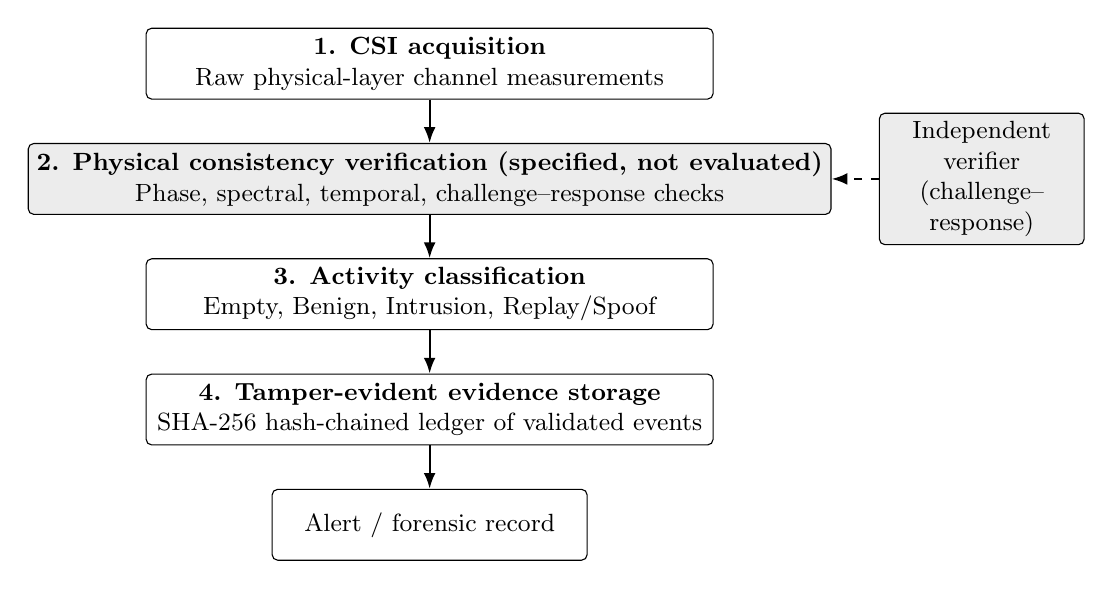
\begin{tikzpicture}[
  box/.style={draw, rounded corners=2pt, align=center, font=\small, minimum width=7.2cm, minimum height=0.9cm, inner sep=3pt},
  ver/.style={box, fill=gray!15},
  arr/.style={-{Latex[length=2mm]}, thick},
  node distance=0.55cm]
\node[box] (a) {\textbf{1. CSI acquisition}\\Raw physical-layer channel measurements};
\node[ver, below=of a] (b) {\textbf{2. Physical consistency verification (specified, not evaluated)}\\Phase, spectral, temporal, challenge--response checks};
\node[box, below=of b] (c) {\textbf{3. Activity classification}\\Empty, Benign, Intrusion, Replay/Spoof};
\node[box, below=of c] (d) {\textbf{4. Tamper-evident evidence storage}\\SHA-256 hash-chained ledger of validated events};
\node[box, below=of d, minimum width=4cm] (e) {Alert / forensic record};
\node[ver, right=0.6cm of b, minimum width=2.6cm, minimum height=1.2cm] (v) {Independent\\verifier\\(challenge--\\response)};
\draw[arr] (a) -- (b);
\draw[arr] (b) -- (c);
\draw[arr] (c) -- (d);
\draw[arr] (d) -- (e);
\draw[arr, dashed] (v) -- (b);
\end{tikzpicture}}
\caption{EchoForensics architecture. The verifier is logically independent of the sensing node. Stages 3 and 4 are evaluated in this paper; stage 2 is not.}
\label{fig:arch}
\end{figure}

%==================================================================
\section{Framework}
\subsection{Channel Model and Synthetic Surrogate}
Conceptually, the channel at subcarrier $i$ and time $t$ is a multipath superposition,
\begin{equation}
H(f_i,t)=\sum_{k} a_k(t)\,\exp\!\big(-j2\pi f_i \tau_k(t)\big)+n(t),
\label{eq:csi}
\end{equation}
with complex path gains $a_k(t)$, delays $\tau_k(t)$, and complex Gaussian noise $n(t)$; a human-induced path has bistatic delay $\tau_h(t)=\big(d_{Tx,h}(t)+d_{h,Rx}(t)\big)/c$. Our experiments do \emph{not} implement this model literally. They use a simplified amplitude-only surrogate (Section~V-A), so no phase information is simulated or used.

\subsection{Classifiers}
\emph{Engineered features.} Eight scalar features per window: amplitude mean, variance, skewness, excess kurtosis, mean inter-subcarrier correlation, a Doppler proxy (mean absolute first difference over time), a periodicity score (mean per-subcarrier autocorrelation at a fixed lag of 100 samples), and the maximum per-subcarrier amplitude excursion. \emph{CNN-BiLSTM-Attention.} The input is the $30\times200$ amplitude window with per-subcarrier z-scoring using training-set statistics only. Table~\ref{tab:cnn} gives the architecture used in the reported experiments.

\begin{table}[t]
\caption{CNN-BiLSTM-Attention Configuration}
\label{tab:cnn}
\centering
\small
\begin{tabular}{p{1.6cm}p{5.4cm}}
\toprule
Layer & Configuration \\
\midrule
Input & 30 subcarrier channels $\times$ 200 time samples \\
Conv1D $\times$2 & 48 then 64 filters; kernel sizes 7 and 5; batch norm; ReLU; max pooling (2) \\
BiLSTM & 48 hidden units per direction \\
Attention & Additive temporal attention \\
Dense head & 48-unit hidden layer; ReLU; dropout 0.25 \\
Output & Four-class softmax \\
\bottomrule
\end{tabular}
\end{table}

\subsection{Tamper-Evident Ledger}
Each validated event record is serialised canonically and chained as
\begin{equation}
h_i=\mathrm{SHA256}\big(\mathrm{payload}_i \,\|\, h_{i-1}\big),
\label{eq:hash}
\end{equation}
where $\|$ is concatenation and $h_{-1}$ is a fixed genesis value ($64$ zeros). Verification recomputes the chain; a modified earlier payload changes its hash, later links diverge, and the first divergence identifies the earliest affected record. This local chain gives evidence of modifications that break the chain but not multi-party non-repudiation.

\subsection{Active Verification Protocol (Specification Only)}
The verifier would issue unpredictable sounding frames and check consistency across phase progression, temporal periodicity, Doppler characteristics, and challenge-conditioned response matching, making substitution of recorded data difficult. It is not implemented or evaluated here. A practical verifier cannot derive an exact expected CSI tensor from a challenge alone, since the channel depends on hardware and environment; it would need calibration or a learned channel model.

%==================================================================
\section{Experimental Protocol}
\subsection{Synthetic Benchmark}
Data are produced by a surrogate generator (30 subcarriers, 200 samples at 100\,Hz, i.e.\ 2\,s windows) that draws everything sequentially from one seeded NumPy generator. For each of 600 \emph{scene groups} it creates one window of each class:
\begin{itemize}
\item \textbf{Scene.} Static profile from four paths with gains $\mathcal{U}(0.25,1)$, phases $\mathcal{U}(0,2\pi)$, and per-subcarrier phase slopes $\mathcal{U}(-0.18,0.18)$, power-normalised.
\item \textbf{Noise.} Complex Gaussian, standard deviation $0.025$ per component; the window amplitude $|H|$ is the model input.
\item \textbf{Empty.} Static profile plus noise.
\item \textbf{Benign.} Adds a path of gain $0.30$ whose phase follows an in-place displacement $\mathcal{U}(0.05,0.25)$\,m sinusoid at $\mathcal{U}(0.3,1.2)$\,Hz with random phase.
\item \textbf{Intrusion.} A crossing with speed $\mathcal{U}(0.6,2.2)$\,m/s, Gaussian envelope (centre $\mathcal{U}(0.35,1.65)$\,s, width $\mathcal{U}(0.08,0.24)$\,s), moving-path gain $0.85$, and attenuation of the static path by up to $48\%$ during the crossing.
\item \textbf{Replay/Spoof.} A segment of length $\mathcal{U}\{20,\dots,60\}$ samples (0.2--0.6\,s) is taken at a random start from the same scene's Empty or Benign window (probability $0.5$ each), tiled to 200 samples, and independent Gaussian noise (standard deviation $0.012$) is added to the amplitude.
\end{itemize}
The result is 2,400 windows (600 per class). The simulator omits AGC variation, CFO, phase noise, interference, and environmental drift.

\subsection{Leakage-Controlled Split and Audit}
Because a replay window is copied from a window of its own scene, all four windows of a scene (its group) are assigned together to one split. Groups are shuffled with a seed-derived generator and split $382/68/150$ groups, giving $1{,}528/272/600$ windows with exactly balanced classes in every split. For every seed the code asserts, and records in a per-seed audit file, that (i) group sets are pairwise disjoint, (ii) every group's four windows lie in one split, and (iii) all 2,400 windows are byte-wise unique (SHA-256 of the raw array), so no identical window crosses a split. These checks do not exclude near-duplicates or generator-induced similarity across scenes. Normalisation statistics and classifier fitting use the training split only.

\subsection{Models and Training}
All models are evaluated on the same splits and seeds. \emph{SVM (mean/var).} A replication of the Wi-Alarm feature set~\cite{wang2019wialarm}: amplitude mean and variance, standardised, RBF kernel, $C=0.8$, $\gamma=20$. \emph{SVM (8 features)} and \emph{Random Forest (8 features)}: standardised RBF SVM with $C=0.8$ and $\gamma=$``scale'', and 200 trees of depth at most 8. \emph{CNN-BiLSTM-Attention:} the architecture specified in Table~\ref{tab:cnn}. The CNN uses Adam (learning rate $10^{-3}$, weight decay $10^{-5}$), batch size 32, cross-entropy loss, and up to 30 epochs with early stopping based on validation loss (patience of 7 epochs); the checkpoint with the lowest validation loss is evaluated. This protocol was fixed before the final runs, no hyperparameter was tuned on the test split, and the test split is used once per seed. Experiments use seeds $11,22,33,44,55$ and are reported as mean $\pm$ standard deviation over seeds.

\subsection{Metrics}
We report accuracy, macro precision, recall and F1, per-class recall, and the macro one-vs-rest AUC. For each class $c$ a binary problem (class $c$ versus the rest) is scored by the softmax or predicted probability $p(c\mid x)$ on the 600 test windows; ROC AUC is computed per class, and the macro value is the unweighted mean. AUC is a ranking metric and can be high even when the decision threshold misses most positives, so per-class recall is reported alongside it.

%==================================================================
\section{Results}
\subsection{Classification Performance}
The five-seed results from the reference implementation are summarised in Table~\ref{tab:perf}. The Random Forest achieves the highest accuracy ($98.87\pm0.48\%$), followed by the RBF SVM ($98.47\pm0.41\%$). The CNN--BiLSTM--Attention model reaches $81.47\pm1.07\%$ accuracy and a macro F1 of $0.7984\pm0.0163$. These results are from the current synthetic benchmark implementation and should not be interpreted as physical Wi-Fi intrusion-detection performance.

\begin{table}[t]
\caption{Classification Performance on the Synthetic Test Split (Mean $\pm$ Standard Deviation over Five Seeds)}
\label{tab:perf}
\centering
\footnotesize
\setlength{\tabcolsep}{2pt}
\resizebox{\columnwidth}{!}{%
\begin{tabular}{@{}lccc@{}}
\toprule
Model & Accuracy (\%) & Macro F1 & Macro OvR AUC \\
\midrule
RBF SVM, 8 features & $98.47\pm0.41$ & $0.9847\pm0.0041$ & $0.99940\pm0.00036$ \\
Random Forest, 8 features & $98.87\pm0.48$ & $0.9887\pm0.0048$ & $0.99959\pm0.00030$ \\
CNN--BiLSTM--Attention & $81.47\pm1.07$ & $0.7984\pm0.0163$ & $0.94089\pm0.00660$ \\
\bottomrule
\end{tabular}
}
\par\smallskip
\footnotesize AUC denotes the macro one-vs-rest area under the ROC curve.
\end{table}

\subsection{Replay/Spoof Performance in the CNN}
The seed-11 classification report provides a per-class diagnostic rather than a five-seed estimate. On its 600-window test split, the CNN obtains $80.5\%$ accuracy and a macro F1 of $0.7874$. Replay/Spoof recall is $36.0\%$ (54 of 150 windows): 86 replay windows are classified as Empty and 10 as Benign. By comparison, Empty recall is $99.3\%$, Benign recall is $88.7\%$, and Intrusion recall is $98.0\%$. These seed-specific results illustrate a replay-class weakness but should not be generalized as five-seed per-class estimates.

\begin{table}[t]
\caption{CNN Per-Class Results for Seed 11}
\label{tab:cnnclass}
\centering
\small
\begin{tabular}{lccc}
\toprule
Class & Precision & Recall & F1 \\
\midrule
Empty & 0.629 & 0.993 & 0.770 \\
Benign & 0.911 & 0.887 & 0.899 \\
Intrusion & 1.000 & 0.980 & 0.990 \\
Replay/Spoof & 0.771 & 0.360 & 0.491 \\
\bottomrule
\end{tabular}
\end{table}

\begin{table}[t]
\caption{CNN Confusion Matrix for Seed 11 (600 Test Windows; Rows = True)}
\label{tab:cm}
\centering
\small
\begin{tabular}{lcccc}
\toprule
 & Empty & Benign & Intrusion & Replay/Spoof \\
\midrule
Empty & 149 & 0 & 0 & 1 \\
Benign & 2 & 133 & 0 & 15 \\
Intrusion & 0 & 3 & 147 & 0 \\
Replay/Spoof & 86 & 10 & 0 & 54 \\
\bottomrule
\end{tabular}
\end{table}

\subsection{Training Behaviour}
The CNN--BiLSTM--Attention model achieves a mean test accuracy of $81.47\pm1.07\%$ and macro F1 of $0.7984\pm0.0163$ over five seeds. Training uses early stopping based on validation loss, with a maximum of 30 epochs. The current experiment outputs do not establish whether the observed performance is caused by underfitting, optimisation, model capacity, or the amplitude-only input representation; these explanations require controlled follow-up experiments.

\subsection{Temporal-Difference Feature Diagnostic}
The synthetic replay generator constructs replay windows by tiling a short segment and adding noise. Across seeds 11, 22, 33, 44, and 55, the temporal-difference feature (mean absolute first difference over time) has a Replay/Spoof-versus-Empty AUC of approximately $1.000$ in the diagnostic analysis. This feature is a proxy derived from synthetic amplitude sequences, not a direct physical Doppler measurement. The result suggests that the generator may introduce a class-specific temporal signature; it does not establish that physical replay attacks are similarly separable.

\subsection{Feature Ablation}
To quantify the contribution of the temporal-difference feature, we reran the feature-based models with all eight features and with that feature removed, using the same five seeds and group-wise split procedure. Table~\ref{tab:ablation} shows a substantial performance reduction when the feature is removed. For the Random Forest, mean accuracy decreases from $98.87\pm0.48\%$ to $82.90\pm1.47\%$, while Replay/Spoof recall decreases from $99.47\pm0.56\%$ to $48.67\pm4.83\%$. For the RBF SVM, accuracy decreases from $98.47\pm0.41\%$ to $77.57\pm0.78\%$. This sensitivity supports treating the high scores as generator-dependent results rather than evidence of robust physical replay detection.

\begin{table}[t]
\caption{Five-Seed Feature Ablation Results (Mean $\pm$ Standard Deviation)}
\label{tab:ablation}
\centering
\scriptsize
\setlength{\tabcolsep}{2pt}
\resizebox{\columnwidth}{!}{%
\begin{tabular}{@{}llccc@{}}
\toprule
Feature set & Model & Accuracy (\%) & Macro F1 & Replay recall (\%) \\
\midrule
All 8 features & Random Forest & $98.87\pm0.48$ & $0.9887\pm0.0048$ & $99.47\pm0.56$ \\
Without temporal difference & Random Forest & $82.90\pm1.47$ & $0.8177\pm0.0163$ & $48.67\pm4.83$ \\
All 8 features & RBF SVM & $98.47\pm0.41$ & $0.9847\pm0.0041$ & $98.27\pm0.37$ \\
Without temporal difference & RBF SVM & $77.57\pm0.78$ & $0.7442\pm0.0107$ & $26.67\pm3.20$ \\
\bottomrule
\end{tabular}
}
\end{table}

\subsection{Synthetic Noise Robustness}
We evaluated the trained CNN on the seed-11 synthetic test inputs after adding zero-mean Gaussian noise at several amplitudes. Table~\ref{tab:noise} reports this single-seed diagnostic. Accuracy decreases from $80.50\%$ at $\sigma=0.005$ to $74.50\%$ at $\sigma=0.25$. Because these perturbations are applied to synthetic amplitudes, the experiment is not a calibrated signal-to-noise ratio study and does not establish robustness on physical CSI. Feature-based model robustness was not evaluated in this experiment.

\begin{table}[t]
\caption{CNN Noise Robustness on the Synthetic Test Split (Seed 11)}
\label{tab:noise}
\centering
\footnotesize
\setlength{\tabcolsep}{3pt}
\begin{tabular}{@{}lcccccc@{}}
\toprule
Noise $\sigma$ & 0.005 & 0.03 & 0.06 & 0.12 & 0.18 & 0.25 \\
\midrule
Accuracy (\%) & 80.50 & 80.17 & 80.33 & 79.50 & 78.17 & 74.50 \\
\bottomrule
\end{tabular}
\end{table}

\subsection{Ledger Tamper Test}
We create a chain of five records, change the confidence of the third from 0.97 to 0.10 without recomputing later hashes, and re-verify. The unmodified chain passes and the modified chain is rejected with the first divergence at (zero-based) index 2. This confirms detection within the tested chain only.

%==================================================================
\section{Security Interpretation}
The results support three limited conclusions. First, on this synthetic benchmark, the Random Forest and RBF SVM using engineered features outperform the CNN--BiLSTM--Attention model. Second, the ablation study shows that removing the temporal-difference feature substantially reduces feature-model performance, indicating strong dependence on a generator-sensitive feature rather than demonstrating robust physical replay detection. Third, the hash-chain software test detects a targeted modification to a stored record when subsequent hashes are not recomputed. The experiments do not establish protection against complete chain reconstruction, label suppression, fabricated CSI, or challenge--response attacks. Real-device CSI collection and physical replay testing remain necessary.

%==================================================================
\section{Limitations}
\textbf{Synthetic, amplitude-only data.} All results come from a surrogate generator without phase, automatic gain control (AGC), carrier frequency offset (CFO), phase noise, interference, or environmental drift.

\textbf{Replay generator and scene variety.} Replay is simulated by tiling a segment and adding noise. The diagnostic suggests that this construction is relatively easy to distinguish. More realistic replay attacks that smooth transitions, match noise statistics, or resynthesise the channel have not been modelled. The scenes also share one parametric family, one person-path model, and one room-independent noise level; multi-person, pet, and through-wall scenarios are absent.

\textbf{CNN performance and explainability.} The cause of the CNN's weak performance has not been established, and the training regimes evaluated are limited. Grad-CAM and SHAP results from earlier drafts were not reproduced and are not claimed in this paper.

\textbf{Verifier not evaluated.} The challenge--response protocol remains a proposal. Its evaluation requires a wireless testbed, calibration, and controlled attacks.

\textbf{Ledger security scope.} A hash chain detects modifications that break the verified chain, but an attacker controlling the entire ledger could rebuild a consistent chain. An independently maintained external anchor is required for stronger protection.

\textbf{Hardware validation.} Future work should evaluate real CSI traces from platforms such as Intel 5300, ESP32, or Nexmon-based systems~\cite{gringoli2019} across rooms, subjects, and days, including physical replay and adversarial attacks.

\section{Conclusion}
This study presents EchoForensics as a proposed zero-trust framework for Wi-Fi CSI-based physical intrusion detection and tamper-evident evidence handling. In the current five-seed synthetic benchmark, the Random Forest achieves $98.87\pm0.48\%$ accuracy and the RBF SVM achieves $98.47\pm0.41\%$, while the CNN--BiLSTM--Attention model achieves $81.47\pm1.07\%$. Feature ablation shows that removing the temporal-difference feature substantially reduces the performance of the feature-based classifiers, highlighting a dependency on the synthetic replay-generation process. The hash-chain demonstration detects a targeted record modification when subsequent hashes are not recomputed. These findings are limited to a synthetic amplitude-only benchmark and a software integrity test; they do not establish real-world intrusion-detection performance or evaluate the proposed challenge--response verifier. Future work will require realistic replay generation, physical Wi-Fi CSI collection, controlled adversarial testing, and independent evidence anchoring.

\section*{Reproducibility Statement}
The synthetic benchmark and the experimental setup are described in this paper. The reported results were obtained using five random seeds (11, 22, 33, 44, and 55). The public reference implementation is available at \url{https://github.com/0xDEADVrm/echoforensics}. The repository should be consulted alongside the manuscript; exact reproducibility requires the published code, configuration, and saved outputs to match the experimental settings reported here. The challenge--response verifier has not been implemented or experimentally evaluated.

\section*{Acknowledgment}
The authors thank the Department of Computer Science and Engineering, Panimalar Engineering College, Chennai, India, for the research facilities and support.

%==================================================================
\begin{thebibliography}{99}
\bibitem{halperin2011} D. Halperin, W. Hu, A. Sheth, and D. Wetherall, ``Tool release: Gathering 802.11n traces with channel state information,'' \emph{ACM SIGCOMM Comput. Commun. Rev.}, vol. 41, no. 1, p. 53, 2011.
\bibitem{wang2014eeyes} Y. Wang, J. Liu, Y. Chen, M. Gruteser, J. Yang, and H. Liu, ``E-eyes: Device-free location-oriented activity identification using fine-grained WiFi signatures,'' in \emph{Proc. ACM MobiCom}, 2014, pp. 617--628.
\bibitem{kotaru2015spotfi} M. Kotaru, K. Joshi, D. Bharadia, and S. Katti, ``SpotFi: Decimeter level localization using WiFi,'' in \emph{Proc. ACM SIGCOMM}, 2015, pp. 269--282.
\bibitem{yousefi2017} S. Yousefi, H. Narui, S. Dayal, S. Ermon, and S. Valaee, ``A survey on behavior recognition using WiFi channel state information,'' \emph{IEEE Commun. Mag.}, vol. 55, no. 10, pp. 98--104, 2017.
\bibitem{ma2019} Y. Ma, G. Zhou, and S. Wang, ``WiFi sensing with channel state information: A survey,'' \emph{ACM Comput. Surv.}, vol. 52, no. 3, Art. no. 46, 2019.
\bibitem{qian2014pads} K. Qian, C. Wu, Z. Yang, Y. Liu, and Z. Zhou, ``PADS: Passive detection of moving targets with dynamic speed using PHY layer information,'' in \emph{Proc. IEEE ICPADS}, 2014, pp. 1--8.
\bibitem{wang2019wialarm} T. Wang, D. Yang, S. Zhang, Y. Wu, and S. Xu, ``Wi-Alarm: Low-cost passive intrusion detection using WiFi,'' \emph{Sensors}, vol. 19, no. 10, Art. no. 2335, 2019.
\bibitem{lundberg2017} S. M. Lundberg and S.-I. Lee, ``A unified approach to interpreting model predictions,'' in \emph{Adv. Neural Inf. Process. Syst.}, 2017, pp. 4765--4774.
\bibitem{selvaraju2017} R. R. Selvaraju, M. Cogswell, A. Das, R. Vedantam, D. Parikh, and D. Batra, ``Grad-CAM: Visual explanations from deep networks via gradient-based localization,'' in \emph{Proc. IEEE ICCV}, 2017, pp. 618--626.
\bibitem{lone2019} A. H. Lone and R. N. Mir, ``Forensic-chain: Blockchain based digital forensics chain of custody with PoC in Hyperledger Composer,'' \emph{Digital Investigation}, vol. 28, pp. 44--55, 2019.
\bibitem{choudhary2023} A. Choudhary, ``Forensic investigations and computer forensics in the age of blockchain,'' \emph{ISACA Journal}, vol. 5, 2023. % VERIFY volume/issue
\bibitem{rose2020zta} S. Rose, O. Borchert, S. Mitchell, and S. Connelly, ``Zero Trust Architecture,'' NIST Special Publication 800-207, 2020.
\bibitem{dehmollaian2020} E. Dehmollaian, B. Etzlinger, N. Ballber Torres, and A. Springer, ``Using channel state information for physical tamper attack detection in OFDM systems: A deep learning approach,'' arXiv:2011.03573, 2020.
\bibitem{basha2024} N. Basha, B. Hamdaoui, A. Erbad, and M. Guizani, ``On the detection of replay authentication attacks through channel state information analysis,'' in \emph{Proc. IEEE GLOBECOM}, 2024, pp. 1719--1724.
\bibitem{lakshmanan2019surfi} N. Lakshmanan, I. Bang, M. S. Kang, J. Han, and J. T. Lee, ``SurFi: Detecting surveillance camera looping attacks with Wi-Fi channel state information,'' in \emph{Proc. ACM WiSec}, 2019, pp. 239--244.
\bibitem{gopalakrishnan2025} S. K. Gopalakrishnan and S. Hailes, ``Towards trustworthy Wi-Fi CSI-based sensing: Systematic evaluation of adversarial robustness,'' arXiv:2511.20456, 2025.
\bibitem{duan2026wiid} Y.-R. Duan, S. Yang, H.-Y. Zhai, X.-Y. Wang, J.-S. Tan, Y.-S. Luo, and S. Chen, ``WiIID: Wi-Fi based intelligent indoor intrusion detection with tensor decomposition,'' \emph{IEEE Wireless Commun. Lett.}, vol. 15, pp. 146--150, 2026.
\bibitem{xu2022wicam} L. Xu, X. Zheng, X. Li, Y. Zhang, L. Liu, and H. Ma, ``WiCAM: Imperceptible adversarial attack on deep learning based WiFi sensing,'' in \emph{Proc. IEEE SECON}, 2022, pp. 10--18.
\bibitem{liu2024time} J. Liu, Y. He, C. Xiao, J. Han, and K. Ren, ``Time to think the security of WiFi-based behavior recognition systems,'' \emph{IEEE Trans. Dependable Secure Comput.}, vol. 21, no. 1, pp. 449--462, 2024.
\bibitem{chen2018ablstm} Z. Chen, L. Zhang, C. Jiang, Z. Cao, and W. Cui, ``WiFi CSI based passive human activity recognition using attention based BLSTM,'' \emph{IEEE Trans. Mobile Comput.}, vol. 18, no. 11, pp. 2714--2724, 2019.
\bibitem{hernandez2020} S. M. Hernandez and E. Bulut, ``Performing WiFi sensing with off-the-shelf smartphones,'' in \emph{Proc. IEEE PerCom Workshops}, 2020, p. 393.
\bibitem{schneier1999} B. Schneier and J. Kelsey, ``Secure audit logs to support computer forensics,'' \emph{ACM Trans. Inf. Syst. Secur.}, vol. 2, no. 2, pp. 159--176, 1999.
\bibitem{syed2022zta} N. F. Syed, S. W. Shah, A. Shaghaghi, A. Anwar, Z. Baig, and R. Doss, ``Zero Trust Architecture (ZTA): A comprehensive survey,'' \emph{IEEE Access}, vol. 10, pp. 57143--57179, 2022.
\bibitem{gringoli2019} F. Gringoli, M. Schulz, J. Link, and M. Hollick, ``Free your CSI: A channel state information extraction platform for modern Wi-Fi chipsets,'' in \emph{Proc. ACM WiNTECH}, 2019, pp. 21--28.
\bibitem{li2017aralarm} S. Li, X. Li, K. Niu, H. Wang, Y. Zhang, and D. Zhang, ``AR-Alarm: An adaptive and robust intrusion detection system leveraging CSI from commodity Wi-Fi,'' in \emph{Enhanced Quality of Life and Smart Living (ICOST)}. Springer, 2017, pp. 211--223.
\end{thebibliography}

\end{document}
